
%%%%%%%%%%%%%%%%%%%%%
\chapter{Système physique et grandeur physique}
%%%%%%%%%%%%%%%%%%%%%
%

\section{Exemple}

Le train parcourt la distance séparant les deux arbres. Cette distance peut être mesurée. La durée pendant laquelle se fait ce déplacement peut être également être mesurée.

\section{Grandeur physique}
  \subsection{Exemples}

Une règle graduée permet de mesurer une longueur. Une horloge permet de mesurer une durée. L'horloge et la règle sont des appareils de mesure. La longueur et la durée sont des grandeurs physiques.

  \subsection{Définitions}

%Un appareil de mesure d'associer une valeur numérique à une réalité physique.

 permet de mesurer une grandeur physique,

\section{Système physique et expérience}

Un système physique est constitué par les objets pris en compte par le physicien lors d'une expérience.

\section{Énergie}
%%\index{energie@énergie}

L'énergie est une {\it grandeur physique}. Elle est déterminée généralement par un calcul à partir d'autre grandeurs qui sont elles mesurables.

\subsection{Énergie}

L'énergie est une grandeur physique fondamentale. L'exemple précédent nous permet d'illustrer les conversions et les transfert d'énergie : Au départ, la balle possède une énergie potentielle de pesanteur due à son altitude. Lorsque la balle tombe, son altitude diminue et sa vitesse augmente : son énergie potentielle est convertie en énergie cinétique.
Lorsque la balle frappe la surface de l'eau, l'onde circulaire se forme : l'énergie cinétique de la balle se convertie en énergie cinétique et potentielle de l'eau. L'onde produite transporte l'énergie dans la mare.

\vspace{0.5cm}
\begin{minipage}[c]{.45\linewidth}
Après avoir touché la surface de l'eau, la balle communique son énergie à l'eau en effectuant quelques oscillations.
De l'énergie est transférée horizontalement dans la mare alors que le mouvement de l'eau correspond à des oscillations verticales.
\end{minipage}
\hfill
\begin{minipage}[c]{.45\linewidth}

%%%%%%%%%%%%%%%%%%%%%        PERSONNAGE AU BORD D'UNE MARE
%

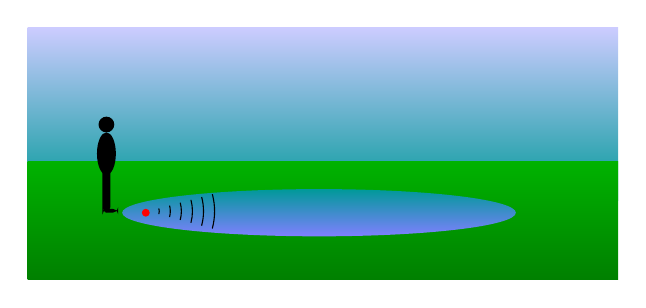
\begin{tikzpicture}
    %  Ciel
  \shade[bottom color=cyan!60!black, top color=blue!20!white] (0,0) rectangle (7.5,2.2);
    %  Sol
  \shade[bottom color=green!50!black, top color=green!70!black] (0,0.5) rectangle (7.5,-1);
    %  Mare
  \shade[bottom color=blue!50!white, top color=cyan!60!black] (3.7,-0.15) ellipse (2.5 and 0.3);
    %  Arbre
 % \pic at (2,2)    {arbre};

    %  Personnage
  \begin{scope}[xshift=1 cm,yshift=0.6 cm]
    % corps et tête
 \fill [black] (0,0)ellipse(0.12 and 0.27);
 \fill [black](0,0.37)circle(0.1);
    % jambe et pieds
 \fill [rounded corners=2pt] (0.05,-0.15)rectangle(-0.05,-0.75);
 \fill [rounded corners=2pt] (0.15,-0.7)rectangle(-0.05,-0.75);
    % bras
 %\fill [rounded corners=2pt, rotate=-15] (-0.1,0.22)rectangle(0.28,0.15);
 %\fill [rounded corners=2pt] (0.22,0.08)rectangle(0.5,0.14);
   % Balle
 \fill[red] (0.5,-0.75) circle(0.05);
  \end{scope}

    %  vague 001
\draw[decorate,decoration={expanding waves,angle=15,segment length=4pt}, rotate=7.5] (1.5,-0.33) -- (2.4,-0.45);

\end{tikzpicture}

%%%%%%%%%%%%%%%%%%%%%%%%%%%%%%%%%%%%%%%%%%%%%%%%%%%%%%%%%%%%%%%%%%%%%%%%%%%%%%%%

\end{minipage}


%
  \subsection{Formes de l'énergie}

Le physicien distingue différentes forme d'énergie :

	\begin{itemize}[leftmargin=1cm, label=\ding{32}, itemsep=1pt]
		\item Cinétique : liée à la vitesse
		\item Potentielle : liée aux interactions conservative
		\item Thermique : liée 
		\item Chimique : liée aux transformations chimiques
		\item De rayonnement : lié aux ondes électromagnétique
	\end{itemize}

L'énergie cinétique est calculée à partir des grandeurs vitesse et masse, 
%
  \subsection{Conservation de l'énergie}

Le principe de conservation de l'énergie est un pilier central de la physique depuis la mécanique classique. Selon ce principe, l'évolution, la transformation, d'un système consiste en une conversion d'une forme de l'énergie en une autre, au cours de ces conversion, l'énergie totale est conservé.

\section{Observable et physique quantique}
%
Les grandeurs mesurées

%%%%%%%%%%%%%%%%%%%%%%%%%%%%%%%%%%%%%%%%%%%%%%%%%%%%%%%%%%%%%%%%%%%%%%%%%%%%%%%%
